\documentclass[oneside]{article}

\usepackage{wallpaper}
\usepackage{geometry}
\usepackage[
    unicode=true,
    bookmarks=true,
    bookmarksnumbered=false,
    bookmarksopen=true,
    bookmarksopenlevel=1,
    breaklinks=false,
    pdfborder={0 0 0},
    backref=false,
    colorlinks=false
    ]{hyperref}
\usepackage{lastpage}
\usepackage{hyphenat}
\usepackage{hyphsubst}
\usepackage{tabularx}
\usepackage{moresize}
\usepackage[document]{ragged2e}
% \usepackage{parskip}

\usepackage[scaled]{helvet}
\usepackage{fontawesome5}
\usepackage[defaultfam,tabular,oldstyle]{montserrat}
\usepackage[T1]{fontenc}
\renewcommand*\oldstylenums[1]{{\fontfamily{Montserrat-TOsF}\selectfont #1}}

\usepackage{titlesec}
\usepackage{xcolor}
\usepackage{tikz}

\setlength{\parindent}{0pt}
\titleformat{\section}{\normalfont}{}{0pt}{}

\renewcommand{\arraystretch}{1.4}

\setlength\fboxrule{0pt}
\setlength\fboxsep{12pt}
% \setlength{\parskip}{.5\baselineskip plus 2pt}
% \renewcommand{\baselinestretch}{1.1}

\titlespacing{\section}{0pt}{1.5ex plus .1ex minus .2ex}{1pc}

\newcolumntype{Y}{>{\RaggedRight\arraybackslash}X}

% Change PDF Meta Info here
\hypersetup{
    pdftitle={Carlos-CV},
    pdfauthor={Carlos Salazar},
    pdfsubject={CV}
}

% Paper size
\geometry{
    a4paper,
    left=0pt,
    right=0pt,
    top=0pt,
    bottom=0pt,
    nohead,
    % includefoot,
    nomarginpar
}

% Background Color of the Sidebar Column
\definecolor{sidebg}{cmyk}{1, 0.02, 0, 0.56}
% Background Color of the Main Column
\definecolor{mainbg}{cmyk}{0, 0, 0.07, 0.04}

% Text Color of the Main Column
\definecolor{maintext}{cmyk}{1, 0.02, 0, 0.8}
% Text Color of the Sidebar Column
\definecolor{sidetext}{cmyk}{0, 0, 0.07, 0.04}

\pagecolor{mainbg}

\begin{document}
\setlength{\topskip}{0pt}\setlength{\footskip}{0pt}%
\fcolorbox{red}{sidebg}{%
    \begin{minipage}[t][\textheight-2\fboxsep-2\fboxrule][t]{\dimexpr0.40\textwidth-2\fboxrule-2\fboxsep\relax}
        \color{sidetext}
        %%%%%%%%%%%%%%%%%%%%%%%%%%%%%%%%%%%%%%%%%%%%%%%%%%%%
        % YOUR NAME, PRONOUNS, OCCUPATION(s), AND HEADSHOT
        {\bfseries\scshape\Huge Carlos Alberto} \\
        {\bfseries\scshape\huge Salazar Martínez} \qquad {Ingeniero Mecatrónico \\ 
        Cedula Profecional: 13570233}
        \vspace{.3cm} \\
        Soy Carlos, un ingeniero mecatrónico con cédula profesional y certificación en diseño mecánico. He trabajado en proyectos en la Secretaría de Infraestructura del Estado de Puebla, automatización y mantenimiento de computadoras, utilizando diversas habilidades técnicas como programación, software de oficina, herramientas de desarrollo, diseño 3D y simulación. Además, cuento con competencias transversales como adaptabilidad, empatía, trabajo en equipo, resiliencia y pensamiento crítico.
        \\
        \begin{center}
            \begin{tikzpicture}
            \clip (0,0) circle (3cm) node[anchor=center] {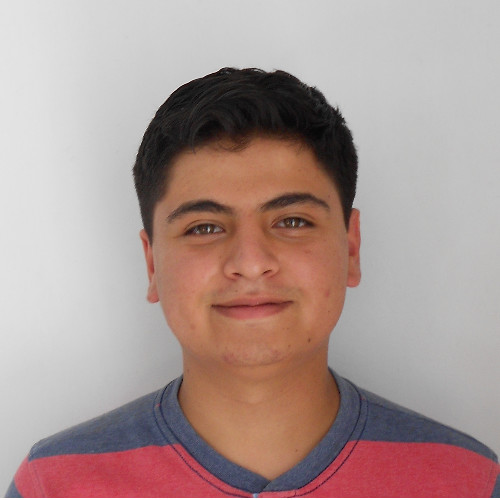
\includegraphics[width=6cm]{imgs/foto.jpg}}; 
            \end{tikzpicture}
        \end{center}
        \vspace{.3cm}
        %%%%%%%%%%%%%%%%%%%%%%%%%%%%%%%%%%%%%%%%%%%%%%%%%%%%
        % YOUR PERSONAL INFROMATION
        \phantomsection{}
        \addcontentsline{toc}{section}{Información Personal}
        \section*{\large Información Personal}
        \begin{tabularx}{\textwidth}{cY}
            \faStarOfLife{} & 16/05/1995 \\
            \faPhone{}      & \href{tel:222-792-1363}{222-792-1363} \\
            \faEnvelope{}   & \href{mailto:carlos.slzrmtz@gmail.com}{carlos.slzrmtz@gmail.com} \\
            \faMapMarker{}  & Av. Dolores Betancourt 210, Contla, Tlatlauquitepec, Puebla, Mexico. C.P. 73900 \\
        \end{tabularx}
        \vspace{.3cm} \\
        \rule{\linewidth}{0.4pt} \\
        %%%%%%%%%%%%%%%%%%%%%%%%%%%%%%%%%%%%%%%%%%%%%%%%%%%%%%%%%
        % YOUR LINKS, YOU MAY ALSO ADD A PERSONAL WEBSITE OR PORTFOLIO
        \phantomsection{}
        \addcontentsline{toc}{section}{Links}
        \section*{\large Links}
        \begin{tabular}{cl}
            \faLinkedin{} & \href{https://www.linkedin.com/in/samcharlie/}{/SamCharlie} \\
            \faGithub{}   & \href{https://github.com/SamCharlie}{/SamCharlie} \\
        \end{tabular}
        \vspace{10pt} \\
        \rule{\linewidth}{0.4pt} \\
        %%%%%%%%%%%%%%%%%%%%%%%%%%%%%%%%%%%%%%%%%%%%%%%%%%%%%%%%%%%%
        % YOUR SKILLS
        % Add/Remove as seen fit, Icons: https://packages.oth-regensburg.de/ctan/fonts/fontawesome5/doc/fontawesome5.pdf
        \phantomsection{}
        \addcontentsline{toc}{section}{Habilidades}
        \section*{\large Habilidades Técnicas}
        \begin{tabularx}{\textwidth}{cY}
            \faCode{}        & C++, C\#, Python, Git\\
            \faFont{}        & Paquetería Office, \LaTeX\\
            \faDesktop{}     & Linux, Windows\\
            \faLaptopCode{}  & VS Code, LabVIEW, Tia Portal V14\\
            \faCogs{}        & SolidWorks, AutoCAD, Catia, Matlab\\
            \faBolt{}        & Proteus, Multisim\\
            \faToolbox{}     & Impresión 3D
        \end{tabularx}
        \vspace{1pt} \\
        \rule{\linewidth}{0.4pt}
        %%%%%%%%%%%%%%%%%%%%%%%%%%%%%%%%%%%%%%%%%%%%%%%%%%%%%%%%%%%%%%%%
        % GRADESCALE (if nesseary, e.g. if you apply abroad, where scales 
        % are different. You should at least provide, what the best possible
        % grade and what the worst possible grade is)
       % \vfill
        %{\tiny Grade scale: (1) very good $\approx$91\%-100\%, (2) good $\approx$81\%-90\%, (3) satisfactory $\approx$66\%-80\%, (4) sufficient $\approx$50\%-65\%, (5) failed $\approx$0\%-49\%}
    \end{minipage}
}
\hfill
\fcolorbox{red}{mainbg}{%
    \begin{minipage}[t][\dimexpr\textheight-2\fboxrule-2\fboxsep\relax][t]{\dimexpr0.6\textwidth-2\fboxrule-2\fboxsep\relax}
        \color{maintext}
        %%%%%%%%%%%%%%%%%%%%%%%%%%%%%%%%%%%%%%%%%%%%%%%%%%%%%%%%%%
        % WORK EXPERIENCE
        \phantomsection{}
        \addcontentsline{toc}{section}{Experiencia de Trabajo}
        \section*{\scshape\Large Experiencia de Trabajo \rule{\linewidth}{0.4pt}}
%
        {\large \textbf{Desarrollo de Infraestructura Téllez}} \\ 
        {{\fontseries{medium}\selectfont Asistente General}} \\
        {\scshape\fontseries{light}\selectfont\footnotesize Nov. 2020 \textendash{} Ago. 2022} \\
        {Jefe Directo: Ing. Juan Manuel Téllez Salazar.} 
        \begin{itemize}
            \setlength{\itemsep}{-3pt}
            \item Supervisor de obras en el municipio de Cuetzalan.
            \item Realización e impresión de planos en AutoCAD.
            \item Creación de un logotipo.
            \item Producción de fotos y videos.
        \end{itemize}
%
        {\large \textbf{Secretaría de Infraestructura del Estado de Puebla}} \\ 
        {{\fontseries{medium}\selectfont Asistente del área de delegados}} \\
        {\scshape\fontseries{light}\selectfont\footnotesize Sep. 2019 \textendash{} Sep. 2020} \\
        {Jefe Directo: Lic. Pedro Martín Hernández Castañeda.} 
        \begin{itemize}
            \setlength{\itemsep}{-3pt}
            \item Creación de un diagnóstico político.
            \item Semaforización de procesos.
            \item Creación de una base de datos para los municipios de Puebla.
        \end{itemize}
%
        {\large \textbf{Desarrollo de Infraestructura Téllez}} \\
        {{\fontseries{medium}\selectfont Prácticas Profesionales}} \\
        {\scshape\fontseries{light}\selectfont\footnotesize Dic. 2017 \textendash{} Dic. 2018} \\
        {Jefe Directo: Ing. Juan Manuel Téllez Salazar.}
        \begin{itemize}
            \setlength{\itemsep}{-3pt}
            \item Capacitación de los trabajadores de obra en EPP.
            \item Realización de planos en AutoCAD.
            \item Asistente en levantamiento topográficos.
        \end{itemize}
%
        {\large \textbf{Secretaría de Educación Pública de Puebla}}\\
        {{\fontseries{medium}\selectfont Servició Social}}\\
        {\scshape\fontseries{light}\selectfont\footnotesize Abr. 2017 \textendash{} Oct. 2017}\\
        {Jefe Directo: Lic. Felicitas Flores Contreras.}
        \begin{itemize}
            \setlength{\itemsep}{-4pt}
            \item Mantenimiento y diagnóstico preventivo de computadoras.
            \item Cambió de suministros de oficina.
            \item Organización de archivo muerto.
            \item Staff en el desfile del 5 mayo.
        \end{itemize}
        %%%%%%%%%%%%%%%%%%%%%%%%%%%%%%%%%%%%%%%%%%%%%%%%%%%%%%%%%%%
        % EDUCATION
        \phantomsection{}
        \addcontentsline{toc}{section}{Educación}
        \section*{\scshape\Large Educación \rule{\linewidth}{0.4pt}}
%
        {\large \textbf{Platzi}} \\
        {\scshape\fontseries{light}\selectfont\footnotesize Online \qquad Nov. 2023 \textendash{} Actual} \\
        {- Ciencia de Datos con Python} \\
        {- Notion}\\
        [2ex]

        {\large \textbf{Licenciatura en Ingeniería Mecatrónica\\ (Universidad del Valle de Puebla)}} \\
        {\scshape\fontseries{light}\selectfont\footnotesize Puebla \qquad Ago. 2014 \textendash{} Ago. 2018} \\
        {Documento obtenido: Titulo y Cedula Profesional.} \\[2ex]

        {\large \textbf{Preparatoria Federal por Cooperación Antonio Audirac}} \\
        {\scshape\fontseries{light}\selectfont\footnotesize Teziutlán, Puebla \qquad Ago. 2011 \textendash{} Ago. 2014} \\
        {Optativa: Diseño} \\[2ex]
        % \\
        \vfill%
        {\hfill\small\fontseries{extralight}\selectfont Page \thepage of \pageref{LastPage}\hfill}
    \end{minipage}
}
\newpage
%%%%%%%%%%%%%%%%%%%%%%%%%%%%%%%%%
% PAGE 2
%%%%%%%%%%%%%%%%%%%%%%%%%%%%%%%%%
\fcolorbox{red}{mainbg}{%
    \begin{minipage}[t][\dimexpr\textheight-2\fboxrule-2\fboxsep\relax][t]{\dimexpr0.6\textwidth-2\fboxrule-2\fboxsep\relax}
        \color{maintext}
        % \vspace{.6cm}
        %%%%%%%%%%%%%%%%%%%%%%%%%%%%%%%%%%%%%%%%%%%%%%%%
        % PROJECTS
        \phantomsection
        \addcontentsline{toc}{section}{Desarrollo Profesional}
        \section*{\scshape\Large Desarrollo Profesional \rule{\linewidth}{0.4pt}}
        \begin{justify}
        \setlength{\parindent}{0pt}

        {\scshape\Large Certificaciones:}\\
        
        \begin{tabularx}{\textwidth}{cY}
            2018 & Certificación en Diseño Mecánico (CSWA) pará el software SolidWorks. \mbox{(C-K7NPBNNR38)} \\
        \end{tabularx}
        \vspace{.2cm}
        \\
        {\scshape\Large Diplomados:}\\

        \begin{tabularx}{\textwidth}{cY}
            2020 & Automatización industrial y CAD / CAM. Tecnológico Nacional de México; Management \& Technology. N° SEP: TECNM-DEC/0613D150/2015-1008. \\
        \end{tabularx}
        \vspace{.2cm}
        \\
        {\scshape\Large Cursos:}\\

        \begin{tabularx}{\textwidth}{cY}
            2024 & Introducción a Inteligencia Artificial (15 h. de teroría y práctica); Platzi. \\
            2023 & Curso de Notion (19 h. de teroría y práctica); Platzi. \\
            2018 & Ford Driving Skills For Life México. Enactus; Ford. \\
            2013 & Taller de soldadura. Tecnológico Superior de Zacapoaxtla. \\
            2013 & Liderazgo e integración y comunicación efectiva. Tecnológico Superior de Zacapoaxtla. \\
        \end{tabularx}

        \end{justify}
        \vfill%
        {\hfill\small\fontseries{extralight}\selectfont Page \thepage of \pageref{LastPage}\hfill}
    \end{minipage}
}
\hfill%
\fcolorbox{red}{sidebg}{%
    \begin{minipage}[t][\dimexpr\textheight-2\fboxrule-2\fboxsep\relax][t]{\dimexpr0.4\textwidth-2\fboxrule-2\fboxsep\relax}
        \color{sidetext}
        % \vspace{.5cm}
        %%%%%%%%%%%%%%%%%%%%%%%%%%%%%%%%%%%%%%%%%%%%%%%%%%%%%%%%
        % YOUR NAME AND PREFERED PRONOUS AGAIN AS HEADER
        {\bfseries\scshape\HUGE Carlos} \\
        {\bfseries\scshape\Huge Salazar} \qquad {Mecatrónico}
        \vspace{.3cm} \\
        %%%%%%%%%%%%%%%%%%%%%%%%%%%%%%%%%%%%%%%%%%%%%%%%%%%%%%%%%%
        % Habilidades blandas
        \phantomsection
        \addcontentsline{toc}{section}{Habilidades blandas}
        \section*{\large Habilidades blandas}
        \begin{tabular}{cl}
            \faDice{} & Adaptabilidad \\
            \faIcon[regular]{handshake} & Empatía \\
            \faIcon{people-carry} & Trabajo en Equipo \\
            \faChartLine{} & Resiliencia \\
            \faBrain{} & Pensamiento Critico
        \end{tabular}
        \vspace{.3cm}
        \\
        \rule{\linewidth}{0.4pt}
        \\
        %%%%%%%%%%%%%%%%%%%%%%%%%%%%%%%%%%%%%%%%%%%%%%%%%%%%%%%%%%
        % LANGUAJES
        \phantomsection
        \addcontentsline{toc}{section}{Languajes}
        \section*{\large Languajes}
        \begin{tabular}{cl}
            \faLanguage{} & Español (Nativa) \\
            \faLanguage{} & English (B1 - TOEFL ITP 456)
        \end{tabular}
        \vspace{.3cm}
        \\
        \rule{\linewidth}{0.4pt}
        \\
        %%%%%%%%%%%%%%%%%%%%%%%%%%%%%%%%%%%%%%%%%%%%
        % HOBBIES
        % Change Icons here https://packages.oth-regensburg.de/ctan/fonts/fontawesome5/doc/fontawesome5.pdf
        \phantomsection
        \addcontentsline{toc}{section}{Hobbies}
        \section*{\large Hobbies}
        \begin{tabularx}{\textwidth}{cY}
            \faCamera{} & Fotografia \\
            \faCogs{} & Realizar proyectos propios \\
        \end{tabularx}
        \vspace{.3cm}
        \\
        \rule{\linewidth}{0.4pt}
    \end{minipage}%
}%
\end{document}